%!TEX program = lualatex
%\documentclass[aspectratio=169,compre%ss,9pt]{beamer}
\documentclass[compress,9pt,xcolor={dvipsnames,table}]{beamer}
\usepackage[T1]{fontenc}
%\usepackage{lmodern}
\usepackage{textcomp}
\usepackage{algorithm}
\usepackage{algorithmic}
\usepackage{tcolorbox}
\usepackage{fontspec}

\usepackage{polyglossia}
\setmainlanguage{english}
\usepackage{tabularx,ragged2e}
\usepackage{booktabs}
\usepackage{dtklogos}
\usepackage{arydshln}
\usepackage{chngpage}

\usepackage{multicol}
\usepackage[caption=false]{subfig}
\hypersetup{%
  colorlinks = true,
  linkcolor  = PineGreen!100!black
}

\usepackage{natbib}

\setbeamertemplate{itemize item}{\color{PineGreen}$\bullet$}
\setbeamertemplate{itemize subitem}{\color{PineGreen!25}$\circ$}
\setbeamercolor{enumerate item}{fg=PineGreen}
\setbeamercolor{caption name}{fg=PineGreen}

\setmainfont[]{Cardo} % sets the roman font
%\setsansfont[]{Alegreya} % sets the sans font % Vallkorn, Alegreya
\setsansfont[]{PT Sans} % sets the sans font
\setmonofont[]{Consolas} % sets the monospace font
\setbeamertemplate{navigation symbols}{}
    \expandafter\def\expandafter\insertshorttitle\expandafter{%
      \insertshorttitle\hfill%
      \insertframenumber\,/\,\inserttotalframenumber}

\usetheme{Szeged}
\usecolortheme{spruce}

\title[Smart usage of context information for the analysis, design and generation of power-aware polices for mobile sensing apps]{ Smart usage of context information for the analysis, design and generation of power-aware polices for mobile sensing apps}
\author[Rafael Perez Torres]{Presented by: Rafael Perez Torres\\[0.5cm] Thesis advisors:\\PhD Cesar Torres Huitzil\\PhD Hiram Galeana Zapien}
\institute{Cinvestav Tamaulipas}
%\date{\today}
\date{}

\begin{document}
\begin{frame}[plain]
  % {
  % \begin{center}
  % 
\includegraphics[scale=0.12]{../../../resources/images/vectors/cinvestav-logo-no-text}
  % \end{center}
  % }
  \begin{center}
  
\includegraphics[scale=0.12]{../../../resources/images/vectors/cinvestav-logo-no-text}
  \end{center}
  \titlepage
  
\end{frame}

%\frame{\maketitle}

\begin{frame}{Table of contents}
	\tableofcontents[hideallsubsections]
\end{frame}

\section{Introduction}
\subsection{Introduction}
\begin{frame}\frametitle{Introduction}
\begin{itemize}
	\item There is a massive adoption of mobile devices by society in almost any daily activity~\cite{Islam2014}.
	\begin{itemize}
		\item Any-where, any-time connectivity
		\item Possibility of installing new mobile applications
		\item Increasing computing, memory, and sensing capabilities
	\end{itemize}
	\item Sensing capabilities of smartphones improve interaction with user, turning mobile devices into \emph{omni-sensors} able to \emph{know} about their surrounding environment.
\end{itemize}
\end{frame}

\begin{frame}\frametitle{Introduction}
\begin{itemize}
	\item Hence, mobile devices have achieved a considerable degree of sensitivity that tries to mimic the sense of humans.
	\item In this way these devices have become \emph{context-aware}, which is translated to an increasing level of understanding about user's activity and environment.
  \item \emph{Context} refers to a four-dimensional space composed of \emph{computing context}, \emph{physical context}, \emph{time context}, and \emph{user context}~\cite{Chen2000}.
\end{itemize}
\end{frame}


\begin{frame}\frametitle{Motivation}
\begin{itemize}
	\item Despite the increasing computing, storage and memory capabilities of smartphones, battery is not evolving at the same pace~\cite{Kjaergaard2012}, growing only 5\% each year~\cite{Ma2012}.
	\item Each new generation of smartphones keeps improving and including new hardware embedded components, which imposes a higher energy demand.
	\item This resource constraint becomes more critical when continuous access to sensors' data is needed, which is the core requirement of \textbf{mobile sensing applications}.
  \item Then it is mandatory for any mobile sensing application development to consider the energy constraint and implement mechanisms or strategies to optimize battery duration.
\end{itemize}
\end{frame}

\begin{frame}\frametitle{Motivation}
\begin{figure}[tb]
  \centering
  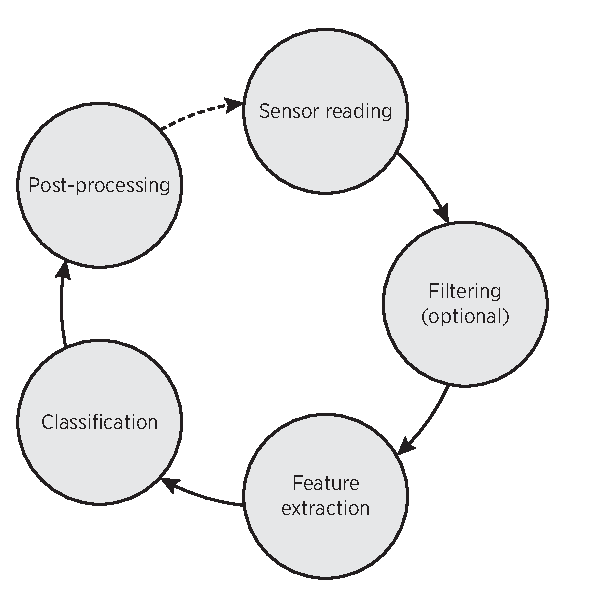
\includegraphics[width=\textwidth]{../../../resources/images/vectors/msa-stages}
  \caption{Stages of mobile sensing applications}
  \label{fig:msa-stages}
\end{figure}

\begin{itemize}
  \item There is a tradeoff between the accuracy of context information retrieved and the associated energy consumption~\cite{Sim2014,Rachuri2012}.
\end{itemize}
\end{frame}


\begin{frame}\frametitle{Motivation}
\begin{figure}[tb]
  \centering
  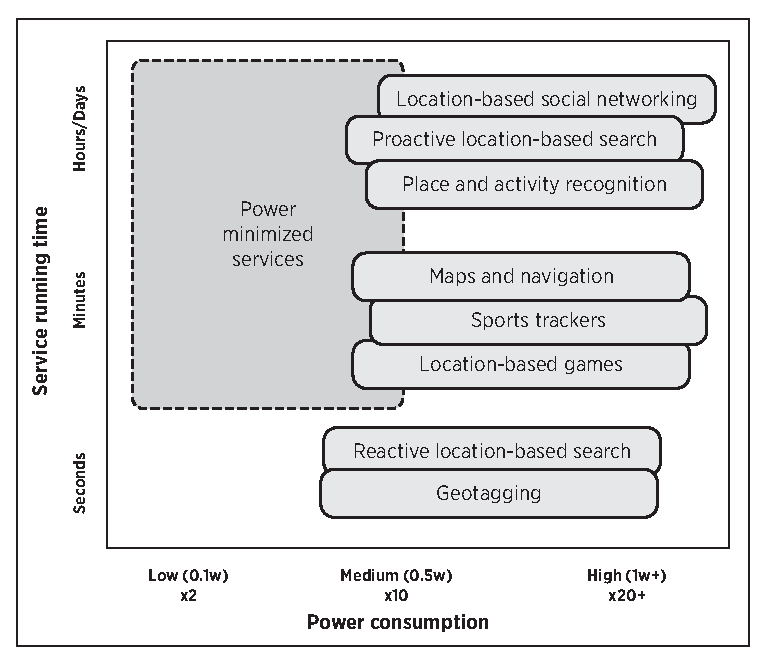
\includegraphics[width=0.65\textwidth]{../../../resources/images/vectors/lbs-classification}
  \caption{Location based services categorization based on running time and power consumption, as proposed by Kj\ae rgaard~\cite{Kjaergaard2012}}.
  \label{fig:lbs-classification}
\end{figure}

\end{frame}

\begin{frame}\frametitle{Basic scenario}
\begin{figure}[tb]
  \centering
  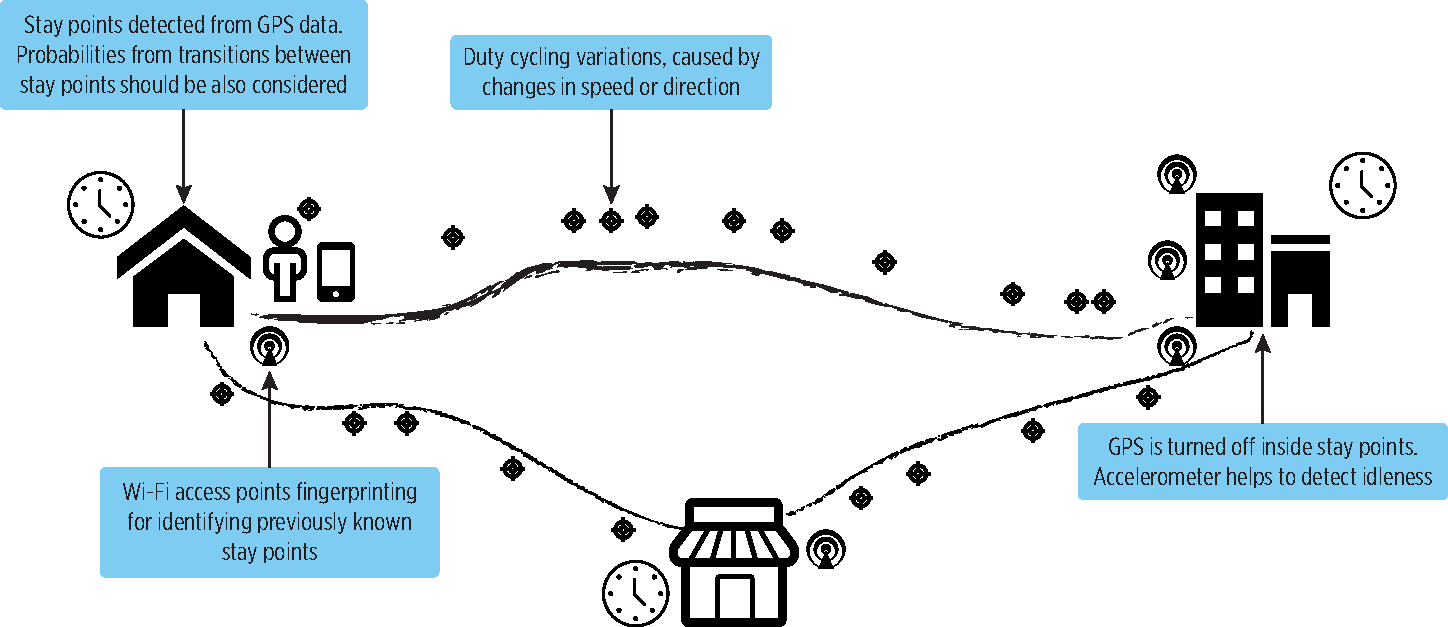
\includegraphics[width=\textwidth]{../../../resources/images/vectors/scenario}
  \caption{Basic scenario}
  \label{fig:scenario}
\end{figure}
\end{frame}

\section{Hypothesis and problem statement}
\subsection{Hypothesis and problem statement}
\begin{frame}\frametitle{Hypothesis}
\begin{tcolorbox}[title=Hypothesis,colframe=PineGreen]
Intelligent policies produced through context information built from sensors data can be employed to reduce the energy consumption in a mobile device when performing continuous sensor readings.
\end{tcolorbox}

{
\small
\begin{itemize}
	\item An intelligent policy is a special rule that defines how sensors should be accessed in order to reduce the energy consumption and achieve the requirements of a mobile app.
	It is intelligent in terms of self-adaptness to changes detected in context information.
	\item This research work aims to employ data coming from GPS and inertial sensors (accelerometer) in order to obtain context information in the shape of user mobility that helps to adapt the usage of sensors and reduce energy consumption.
\end{itemize}
}
\end{frame}


\begin{frame}\frametitle{Problem statement}
\begin{tcolorbox}[title=Problem statement: Mobility pattern identification,colframe=PineGreen]
\small
Given a set $V = \left\{v_{1}, v_{2}, \dotsc, v_{n}\right\}$ of data values read from sensor $S$ in the time interval $T  \in [t_{1}, t_{2}]$, identify the current mobility pattern $p_{S}$ that represents the activity of user.

\begin{equation}
  \text{PatternIdentifier}( V ) \longrightarrow{} p_{S} \in Patterns
\end{equation}

Where $Patterns$ is a set of patterns that represent an interesting state in user mobility, specifically the set $\left\{no\_movement, walking, running, vehicle\_transportation\right\}$.
\end{tcolorbox}
\end{frame}

\begin{frame}\frametitle{Problem statement}
\begin{tcolorbox}[title=Problem statement: Policy generation,colframe=PineGreen]
\small
Given the set of detected mobility patterns $\mathcal{P} = \{ p_{S_1}, p_{S_2}, \ldots, p_{S_n} \}$ in data from sensors $\mathcal{S} = \{ S_1,S_2,\ldots, S_n \}$, parameters for assigning weight to energy $e$ and accuracy $a$, and physical constraints status $c$ of a mobile device, find a policy that select the proper set of sensors $\mathcal{S}_{new}$ and its associated configuration $\mathcal{S}_{new_{conf}}$  while meeting application requirements.

\begin{equation}
  \text{PolicyGeneration}( \mathcal{P}_{\mathcal{S}}, e, a, c ) \longrightarrow{} \mathcal{S}_{new}, \mathcal{S}_{new_{conf}}
\end{equation}

The $\mathcal{S}_{new_{conf}}$ configuration is referred as the \emph{duty cycle} of associated sensor.
\end{tcolorbox}
\end{frame}

\begin{frame}\frametitle{Interaction between problems}
\begin{figure}[tb]
  \centering
  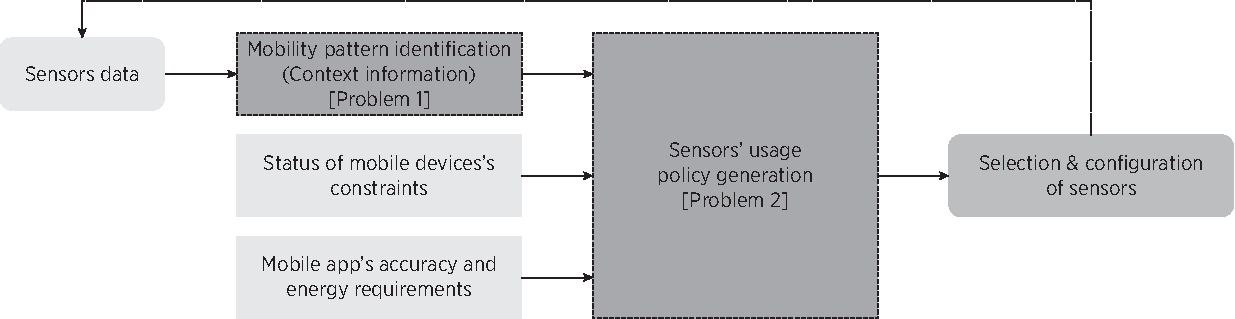
\includegraphics[width=\textwidth]{../../../resources/images/vectors/problems-incorporation}
  \caption{Interaction between the thesis work's problems}
  \label{fig:probems-incorporation}
\end{figure}
\end{frame}

\section{Objectives}
\subsection{Objectives}
\begin{frame}\frametitle{Objectives}
\begin{tcolorbox}[title=Main objective,colframe=PineGreen]
To reduce energy consumption in the mobile sensing apps, which perform continuous sensor readings, through self-adapting power-aware policies generated from context information obtained from sensors data.
\end{tcolorbox}
\end{frame}

\begin{frame}\frametitle{Objectives}
\begin{tcolorbox}[title=Particular objectives,colframe=PineGreen]
\small
\begin{itemize}
  \item To identify mobility patterns from context information obtained from an inertial sensor (accelerometer) and location providers (GPS, WPS).
  \item To generate policies for a self-adapting sensors' usage from identified mobility patterns, accuracy and energy requirements of mobile application, and status of mobile device's constraints. 
  \item To ease the development of mobile sensing applications that require user location tracking, i.e., LBS, isolating the complexity of sensors' access and the associated efficient energy management.
\end{itemize}
\end{tcolorbox}
\end{frame}


\section{Methodology}
\subsection{Methodology}
\begin{frame}\frametitle{Methodology}
\begin{enumerate}
  \item Familiarization with state-of-art power-aware sensing related techniques
  \item Formal definition and selection of mobility patterns to be identified
  \item Research on pattern recognition algorithms focused on mobility patterns identification
  \item Design of the Pattern Identification Element (PIE)
  \item Research on and proposition of adaptive policies for energy efficient usage of sensors
  \item Design of the Policy Generation Element (PGE)
  \item Development of a middleware involving the PIE and PGE for the Android platform
  \item Experimentation in terms of accuracy and energy efficiency
\end{enumerate}
\end{frame}


\section{Schedule}
% ---------------------------------
\subsection{Schedule}
\begin{frame}{Schedule}
  \definecolor{colorA}{gray}{0.85}
  \definecolor{colorB}{gray}{0.95}
  \definecolor{colorStep}{gray}{1}

  \newlength{\longitudCelda}
  \setlength{\longitudCelda}{75mm}

  \begin{table}[!h]
  {
    \scalebox{0.75}{
    \small
      \begin{tabular*}{16.5cm}{lp{\longitudCelda}*{7}{c}}
          & & \multicolumn{1}{ :c: }{\tiny 2014} & \multicolumn{3}{ c: }{\tiny 2015} & \multicolumn{3}{ c: }{\tiny 2016}  \\
          \cline{3-9}

          \multicolumn{2}{c:}{}
          & \multicolumn{1}{c:}{\tiny 3\textsuperscript{rd}} 
          & \tiny 1\textsuperscript{st} & { \tiny 2\textsuperscript{nd}} & \multicolumn{1}{c:}{ \tiny 3\textsuperscript{rd}}
          & \tiny 1\textsuperscript{st} & \tiny 2\textsuperscript{nd} & \multicolumn{1}{c:}{ \tiny 3\textsuperscript{rd}} \\
          \cline{3-9}

          % Step 1
          \rowcolor{colorStep}
          & \multicolumn{1}{c}{\scriptsize \textsc{Step I}}  & & & & & & \\
          
          \rowcolor{colorA}
          1 & \multicolumn{1}{p{\longitudCelda}:}{State-of-art reading} &
          \cellcolor[gray]{0.3} & \cellcolor[gray]{0.3} & &
          & & & \\

          \rowcolor{colorB}
          2 & \multicolumn{1}{p{\longitudCelda}:}{State-of-art works categorization} &
          & \cellcolor[gray]{0.3} & \cellcolor[gray]{0.3} &
          & & & \\

          \rowcolor{colorA}
          3 & \multicolumn{1}{p{\longitudCelda}:}{Documentation of information found (committee request)} &
          & & \cellcolor[gray]{0.3} &
          & & & \\

          % Step 2
          \rowcolor{colorStep}
          & \multicolumn{1}{c}{\scriptsize \textsc{Step II}}  & & & & & & & \\

          \rowcolor{colorB}
          4 & \multicolumn{1}{p{\longitudCelda}:}{Development of a mobile app for the Android platform that collects accelerometer and location data} &
          & & \cellcolor[gray]{0.3} & 
          \cellcolor[gray]{0.3} & & & \\

          \rowcolor{colorA}
          5 & \multicolumn{1}{p{\longitudCelda}:}{Analysis of data delivered by the mobile app} &
          & & & 
          \cellcolor[gray]{0.3} & & & \\

          \rowcolor{colorB}
          6 & \multicolumn{1}{p{\longitudCelda}:}{Creation of the formal definition of mobility pattern} &
          & & &
          \cellcolor[gray]{0.3} & & & \\

          \rowcolor{colorA}
          7 & \multicolumn{1}{p{\longitudCelda}:}{Selection of the mobility patterns to be recognizable by the system} &
          & & & 
          \cellcolor[gray]{0.3} & \cellcolor[gray]{0.3} & & \\

          % Step 3
          \rowcolor{colorStep}
          & \multicolumn{1}{c}{\scriptsize \textsc{Step III}}  & & & & & & & \\

          \rowcolor{colorB}
          8 & \multicolumn{1}{p{\longitudCelda}:}{Research on classification algorithms adequate to work with mobility patterns} &
          & & & 
          \cellcolor[gray]{0.3} & \cellcolor[gray]{0.3} & & \\

          \rowcolor{colorA}
          9 & \multicolumn{1}{p{\longitudCelda}:}{Definition of metrics for evaluating algorithms when executing on a mobile platform} &
          & & & 
          & \cellcolor[gray]{0.3} & & \\

          \rowcolor{colorB}
          10 & \multicolumn{1}{p{\longitudCelda}:}{Implementation of algorithms (including proper adaptions towards running on a mobile platform) for evaluation} &
          & & & 
          & \cellcolor[gray]{0.3} & \cellcolor[gray]{0.3} & \\

          \rowcolor{colorA}
          11 & \multicolumn{1}{p{\longitudCelda}:}{Selection of best algorithms according to metrics} &
          & & & 
          & & \cellcolor[gray]{0.3} & \\


          % Step 4
          \rowcolor{colorStep}
          & \multicolumn{1}{c}{\scriptsize \textsc{Step IV}}  & & & & & & & \\

          \rowcolor{colorB}
          12 & \multicolumn{1}{p{\longitudCelda}:}{Definition and modeling of parameters needed by the PIE} &
          & & & 
          \cellcolor[gray]{0.3} & \cellcolor[gray]{0.3} & \cellcolor[gray]{0.3} &
          \cellcolor[gray]{0.3}\\

          \rowcolor{colorA}
          13 & \multicolumn{1}{p{\longitudCelda}:}{Building of the PIE} &
          & & & 
          \cellcolor[gray]{0.3} & \cellcolor[gray]{0.3} & \cellcolor[gray]{0.3} &
          \cellcolor[gray]{0.3} \\

      \end{tabular*}
    }
  } % begin table
  \caption{Schedule of activities (each column represents a four months period)}
  \label{tbl-schedule}
  \end{table}
\end{frame}


\begin{frame}{Schedule}
  
  \newlength{\longCelda}
  \setlength{\longCelda}{75mm}
  \definecolor{colorA}{gray}{0.85}
  \definecolor{colorB}{gray}{0.95}
  \definecolor{colorStep}{gray}{1}

  \begin{table}[!h]
  {
    \scalebox{0.8}{
    \small
      \begin{tabular*}{16.5cm}{lp{\longCelda}*{6}{c}}
          & & \multicolumn{3}{ :c: }{\tiny 2016} & \multicolumn{3}{ c: }{\tiny 2017} \\
          \cline{3-8}

          \multicolumn{2}{ c: }{}
          & \multicolumn{1}{c}{\tiny 1\textsuperscript{st}} & { \tiny 2\textsuperscript{nd}} & \multicolumn{1}{c:}{ \tiny 3\textsuperscript{rd}}
          & \tiny 1\textsuperscript{st} & \tiny 2\textsuperscript{nd} & \multicolumn{1}{c:}{ \tiny 3\textsuperscript{rd}} \\
          \cline{3-8}

          % Step 5
          \rowcolor{colorStep}
          & \multicolumn{1}{c}{\scriptsize \textsc{Step V}}  & & & & & & \\
          
          \rowcolor{colorA}
          14 & \multicolumn{1}{p{\longCelda}:}{Creation of the formal definition of policy} &
          & & \cellcolor[gray]{0.3} &
          & & \\

          \rowcolor{colorB}
          15 & \multicolumn{1}{p{\longCelda}:}{Research and evaluation of techniques for generation and adaption of policies} &
          & & \cellcolor[gray]{0.3} & 
          \cellcolor[gray]{0.3} & & \\

          \rowcolor{colorA}
          16 & \multicolumn{1}{p{\longCelda}:}{Design and execution of experiments with techniques applied to use cases} &
          & & \cellcolor[gray]{0.3} & 
          \cellcolor[gray]{0.3} & & \\

          \rowcolor{colorB}
          17 & \multicolumn{1}{p{\longCelda}:}{Selection of best techniques} &
          & & &
          \cellcolor[gray]{0.3} & & \\


          % Step 6
          \rowcolor{colorStep}
          & \multicolumn{1}{c}{\scriptsize \textsc{Step VI}}  & & & & & & \\
          
          \rowcolor{colorA}
          18 & \multicolumn{1}{p{\longCelda}:}{Definition and modeling of parameters needed by the PGE} &
          & & &
          & \cellcolor[gray]{0.3} & \\

          \rowcolor{colorB}
          19 & \multicolumn{1}{p{\longCelda}:}{Building of the PGE} &
          & & &
          & \cellcolor[gray]{0.3} & \\



		  % Step 7
          \rowcolor{colorStep}
          & \multicolumn{1}{c}{\scriptsize \textsc{Step VII}}  & & & & & & \\
          
          \rowcolor{colorA}
          20 & \multicolumn{1}{p{\longCelda}:}{Analysis of elements involved into software abstractions} &
          & & &
          & \cellcolor[gray]{0.3} & \\

          \rowcolor{colorB}
          21 & \multicolumn{1}{p{\longCelda}:}{Research on Android API for specialized components} &
          & & &
          & \cellcolor[gray]{0.3} & \\

          \rowcolor{colorA}
          22 & \multicolumn{1}{p{\longCelda}:}{Development of the middleware} &
          & & &
          & \cellcolor[gray]{0.3} & \\


      \end{tabular*}
     }
  } % begin table
  \caption{Schedule of activities (each column represents a four months period)}
  \label{tbl-schedule-2}
  \end{table}
\end{frame}

\begin{frame}{Schedule}
  
  \newlength{\longCell}
  \setlength{\longCell}{75mm}
  \definecolor{colorA}{gray}{0.85}
  \definecolor{colorB}{gray}{0.95}
  \definecolor{colorStep}{gray}{1}

  \begin{table}[!h]
  {
    \scalebox{0.8}{
    \small
      \begin{tabular*}{16.5cm}{lp{\longCell}*{5}{c}}
          & & \multicolumn{3}{ :c: }{\tiny 2017} & \multicolumn{2}{ c: }{\tiny 2018} \\
          \cline{3-7}

          \multicolumn{2}{ c: }{}
          & \multicolumn{1}{c}{\tiny 1\textsuperscript{st}} & { \tiny 2\textsuperscript{nd}} & \multicolumn{1}{c:}{ \tiny 3\textsuperscript{rd}}
          & \tiny 1\textsuperscript{st} & \tiny 2\textsuperscript{nd} \\
          \cline{3-7}

          % Step 8
          \rowcolor{colorStep}
          & \multicolumn{1}{c}{\scriptsize \textsc{Step VIII}}  & & & \\
          
          \rowcolor{colorA}
          23 & \multicolumn{1}{p{\longCell}:}{Definition of experiments targeting accuracy and energy consumption axes} &
          & & \cellcolor[gray]{0.3} &
          & \\

          \rowcolor{colorB}
          24 & \multicolumn{1}{p{\longCell}:}{Development of needed sample mobile apps for running experimentation} &
          & & \cellcolor[gray]{0.3} &
          & \\

          \rowcolor{colorA}
          25 & \multicolumn{1}{p{\longCell}:}{Execution of experimentation} &
          & & \cellcolor[gray]{0.3} &
          \cellcolor[gray]{0.3} & \\

          \rowcolor{colorB}
          26 & \multicolumn{1}{p{\longCell}:}{Results analysis} &
          & & &
          \cellcolor[gray]{0.3} & \\

      \end{tabular*}
     }
  } % begin table
  \caption{Schedule of activities (each column represents a four months period)}
  \label{tbl-schedule-3}
  \end{table}
\end{frame}


\begin{frame}{Schedule}
  
  \newlength{\longCella}
  \setlength{\longCella}{50mm}
  \definecolor{colorA}{gray}{0.85}
  \definecolor{colorB}{gray}{0.95}
  \definecolor{colorStep}{gray}{1}


  \begin{table}[!h]
  {
    \scalebox{0.75}{
    %\scalebox{0.6}{
    \small
      \begin{tabular*}{16.5cm}{lp{\longCella}*{12}{c}}
          & & \multicolumn{1}{ :c: }{\tiny 2014} & \multicolumn{3}{ c: }{\tiny 2015} & \multicolumn{3}{ c: }{\tiny 2016}  & \multicolumn{3}{ c: }{\tiny 2017} & \multicolumn{2}{ c }{\tiny 2018} \\
          \cline{3-14}

          \multicolumn{2}{c:}{}
          & \multicolumn{1}{c:}{\tiny 3\textsuperscript{rd}} 
          & \tiny 1\textsuperscript{st} & { \tiny 2\textsuperscript{nd}} & \multicolumn{1}{c:}{ \tiny 3\textsuperscript{rd}}
          & \tiny 1\textsuperscript{st} & \tiny 2\textsuperscript{nd} & \multicolumn{1}{c:}{ \tiny 3\textsuperscript{rd}}
          & \tiny 1\textsuperscript{st} & \tiny 2\textsuperscript{nd} & \multicolumn{1}{c:}{ \tiny 3\textsuperscript{rd}}
          & \tiny 1\textsuperscript{st} & \tiny 2\textsuperscript{nd} \\
          \cline{3-14}

          % Step 1
          \rowcolor{colorStep}
          & \multicolumn{1}{c}{\scriptsize \textsc{Required tasks}}  & & & & & & & & & & & & \\
          
          \rowcolor{colorA}
          A & \multicolumn{1}{p{\longCella}:}{Related subject courses} &
          \cellcolor[gray]{0.3} & \cellcolor[gray]{0.3} & \cellcolor[gray]{0.3} &
          & & &
          & & &
          & & \\

          \rowcolor{colorB}
          B & \multicolumn{1}{p{\longCella}:}{Research articles submission} &
          & & &
          & & \cellcolor[gray]{0.3} &
          & & \cellcolor[gray]{0.3} &
          & & \\

          \rowcolor{colorA}
          C & \multicolumn{1}{p{\longCella}:}{Thesis writing} &
          \cellcolor[gray]{0.3} & & &
          \cellcolor[gray]{0.3} & & &
          \cellcolor[gray]{0.3} & & &
          \cellcolor[gray]{0.3} & \cellcolor[gray]{0.3} & \cellcolor[gray]{0.3} \\

      \end{tabular*}
    }
  } % begin table
  \caption{Schedule of required activities}
  \label{tbl-schedule-4}
  \end{table}
\end{frame}



\section{Contributions}
\subsection{Contributions}
\begin{frame}\frametitle{Contributions}
\begin{itemize}
  \item A mechanism for detecting mobility patterns from the data read by sensors of mobile devices (especifically GPS and accelerometer).
  \item A mechanism for generating policies for accessing sensors.
  %Besides the identified mobility pattern, such mechanism also considers mobile application's requirements (energy and accuracy hints), and the status of device constraints.
  The produced policies will allow to perform an intelligent usage of smartphone's sensing infrastructure in continuous sensor readings, reducing the energy consumption.
  \item A middleware implementing the previous power-aware mechanisms for easing the development of location based services.
\end{itemize}
\end{frame}

\section{Conclusions}
\subsection{Conclusions}
\begin{frame}\frametitle{Conclusions}
In this talk:
\begin{itemize}
  \item An introduction to the energy consumption issue in mobile sensing apps and its relevance has been presented.
  \item A description of the important components of our thesis work has been also given.
  \item An overview of the proposed methodology for solving the energy consumption issue has been provided.
\end{itemize}
\end{frame}

\begin{frame}\frametitle{}
\begin{center}
{
\Huge
Thank You\\ for your attention!
}
\end{center}

\end{frame}

\subsection{References}
\bibliographystyle{plain}
% \bibliographystyle{unsrtnat}
% \tiny
\bibliography{../../../resources/references/bibliography}


% \section[]*{Developed work}
\subsection*{Developed work}
\begin{frame}\frametitle{Brief state of art revision}
\begin{figure}[tb]
  \centering
  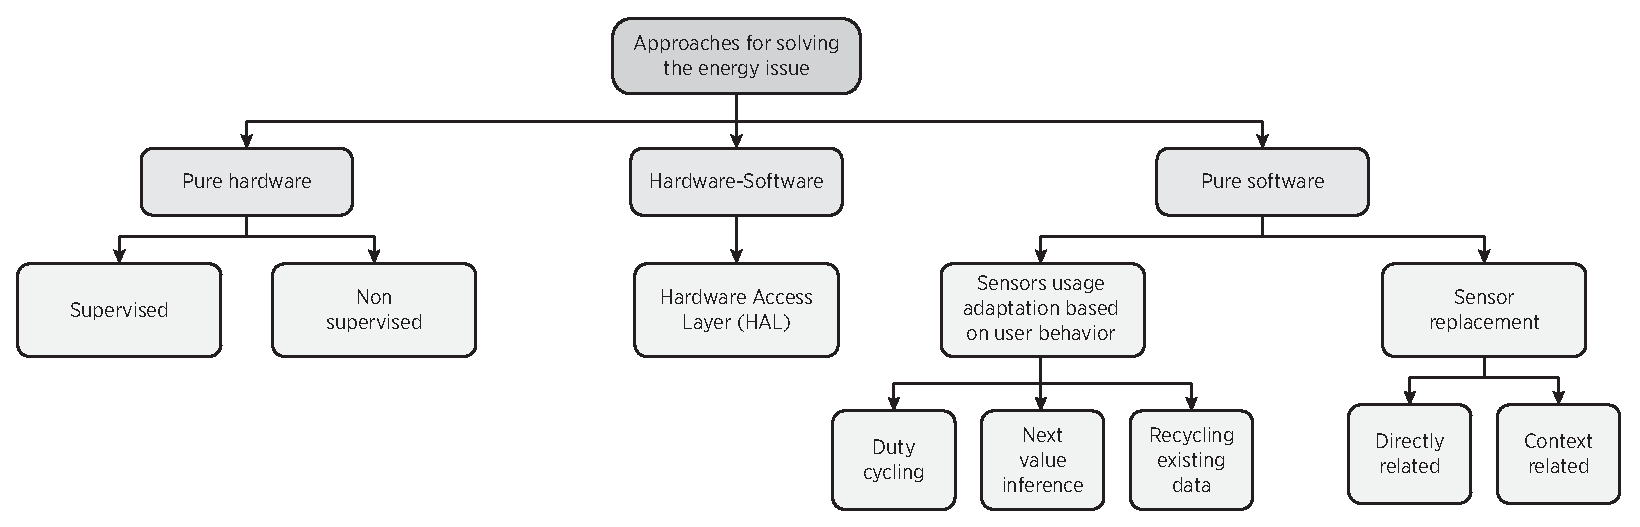
\includegraphics[width=\textwidth]{../../../resources/images/vectors/approaches-taxonomy}
  \caption{Taxonomy of solutions}
  \label{fig:taxonomy}
\end{figure}
\end{frame}

\begin{frame}\frametitle{Brief state of art revision}
\begin{figure}[tb]
  \centering
  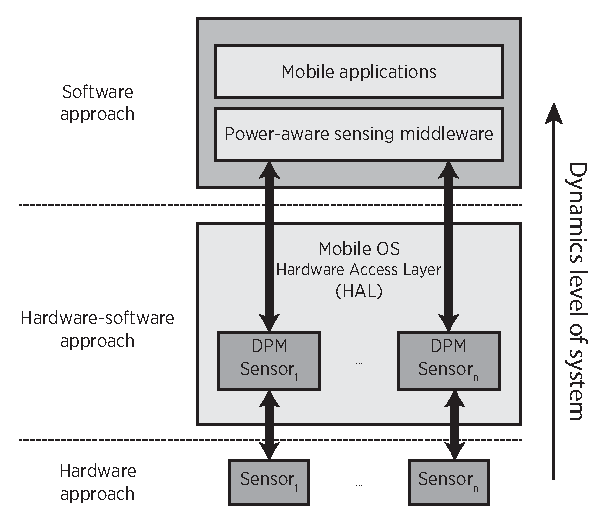
\includegraphics[scale=0.72]{../../../resources/images/vectors/approaches-distribution}
  \caption{Distribution of approaches across mobile platform's layers}
  \label{fig:distribution}
\end{figure}
\end{frame}

\begin{frame}\frametitle{Proposed solution}
\begin{figure}[tb]
  \centering
  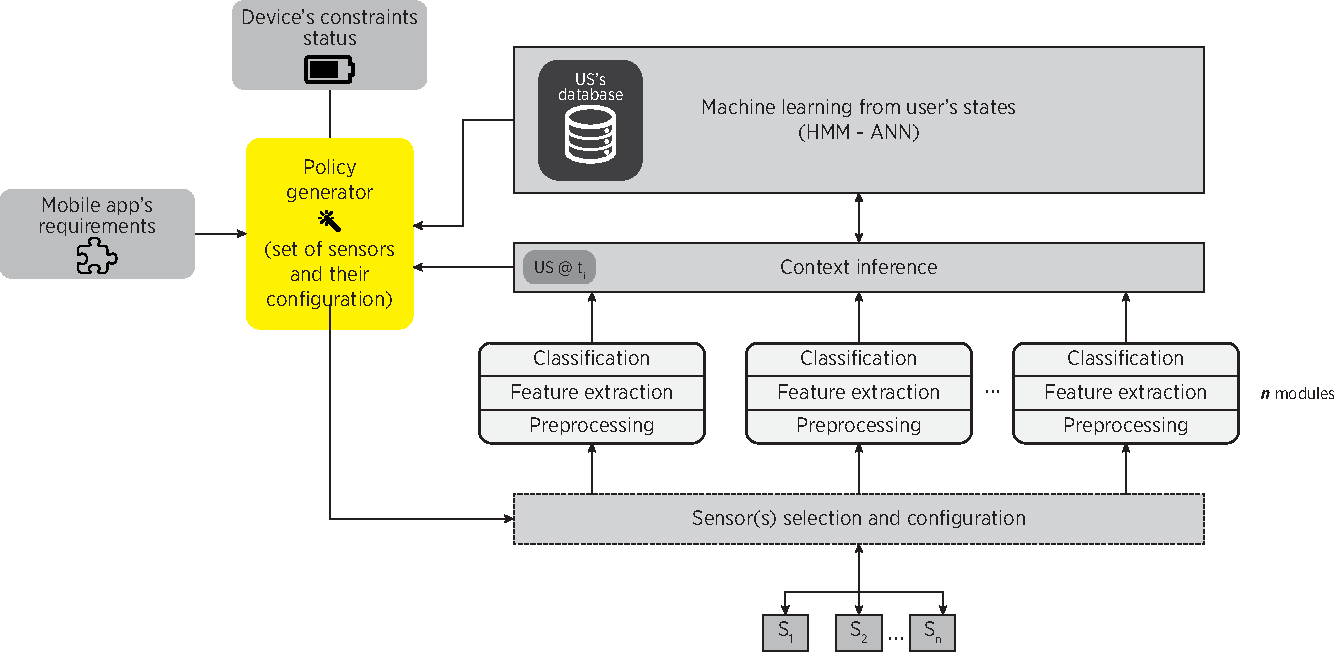
\includegraphics[width=\textwidth]{../../../resources/images/vectors/policy-manager-incorporation}
  \caption{Overview of current solution}
  \label{fig:solution}
\end{figure}
\end{frame}

\end{document}
